\section{Tutorial} \label{section: tutorial}

\subsection{Preparando o Projeto} \label{section: tutorial project setup}

Assegure-se de que tem o Node.js instalado globalmente na sua máquina antes de começarmos; isto permitir-nos-á importar todas as nossas dependências e inicializar o projeto. Além disso, para a base de dados será utilizada uma \textit{cluster} gratuito hospedado no MongoDB Atlas \cite{noauthor_mongodb_nodate-1}, mas poderá, em alternativa, utilizar uma instância local do MongoDB.

Vamos começar por criar uma nova pasta para o projeto, instalar as nossas dependências, e montar a estrutura. No terminal do seu computador execute o seguinte:

\lstinputlisting[language=SH, caption=Comandos para a inicialização do projeto]{Listings/1. Tutorial/project_setup.sh}

Então, linha por linha: (1) criámos a pasta \texttt{api-ementa}, (2) entramos na pasta criada, (3) inicializámos um projeto Node, (4) instalámos o Fastify e o Mongoose como dependências, (5)criámos uma nova pasta \texttt{src} com (6) um ficheiro \texttt{index.js} que será a raiz da nossa aplicação.

\subsubsection{Inicializando o Fastify e Mongoose}

Em seguida, vamos fazer a nossa aplicação Fastify funcionar com a ligação ao MongoDB.

Portanto, no ficheiro \texttt{index.js} que acabamos de criar vamos colocar o seguinte:

\lstinputlisting[language=ES6, caption=Ficheiro index.js inicial]{Listings/1. Tutorial/index_1.js}

Começamos por importar o \texttt{fastify} e \texttt{mongoose} e utilizámos a função \texttt{fastify()} para iniciar a aplicação. Como a função \texttt{mongoose.connect()} nos permite especificar um URI para ligar a nossa base de dados à aplicação, utilizou-se o URI de conexão fornecido pelo MongoDB Atlas na secção de ligações, como dito anteriormente, poderá ser utilizada qualquer instância local ou remota de MongoDB. Deverá ainda de atribuir um nome à base de dados do projeto no final do URI, no caso deste exemplo foi atribuído o nome \texttt{api-ementa}. Poderá atribuir o nome que quiser, se a instância do MongoDB não tiver uma base de dados com esse nome, a mesma será automaticamente criada.

A aplicação trata então da rota principal com a função \texttt{app.get()}. Isto trata de um pedido GET para a raiz da nossa aplicação (\texttt{"/"}). Ao utilizar uma aplicação Fastify para tratar uma rota, devemos fornecer uma função que contenha o \texttt{request} e \texttt{reply} como parâmetros. Como seria de esperar, a primeira contém todos os detalhes do pedido, enquanto a segunda é utilizada para enviar uma resposta formatada para o destino. Por enquanto, simplesmente devolvemos uma string com \texttt{reply.send()}.

Por fim, utilizamos a função \texttt{app.listen} para fazer a nossa aplicação ficar à escuta na porta 8080. Agora é altura de testarmos. Para o fazer, vá até ao ficheiro \texttt{package.json}, na raiz da nossa aplicação, e adicione o seguinte script \texttt{"start"} ao objeto \texttt{"scripts"}:

\lstinputlisting[language=JSON, caption=Ficheiro package.json]{Listings/1. Tutorial/package_1.json}

Agora basta executar \texttt{npm run start} a partir do seu terminal e deverá ver uma mensagem a dizer "Server running on http://127.0.0.1:8080". Abra o seu browser em http://localhost:8080 e deverá ver a nossa string "Server alive!", o que significa que a nossa aplicação está a funcionar!

\subsection{Definindo o Modelo de Dados}

Precisamos de criar uma coleção para os produtos da nossa ementa na nossa base de dados, bem como descrever as características que um documento de produto deve conter. Podemos faze-lo estabelecendo um Modelo de Produto baseado recorrendo a um \texttt{Model Schema}, que é um objeto que contém todas as especificações de um documento normal de um produto. Vamos fazer uma nova pasta e ficheiro dentro do nosso projeto; num terminal dentro da sua pasta de projeto, escreva:

\lstinputlisting[language=SH, caption=Comandos para criar os modelos]{Listings/1. Tutorial/create_models.sh}

Vamos adicionar ao novo ficheiro o seguinte código:

\lstinputlisting[language=ES6, caption=Ficheiro models/product.model.js]{Listings/1. Tutorial/models_product_1.js}

Essencialmente, estamos a utilizar o objeto \texttt{Schema} do Mongoose para dizer a MongoDB que os nossos produtos devem conter uma propriedade obrigatória chamada \texttt{name} do tipo string para o nome do produto, uma propriedade opcional chamada \texttt{description} também do tipo string para a descrição do produto e uma propriedade obrigatória chamada \texttt{price} do tipo número para o preço do produto.

A função \texttt{mongoose.model} é então utilizada para transformar este esquema num modelo. A primeira opção é uma string que MongoDB utilizará para definir o nome da coleção: se tivermos um modelo \texttt{"product"}, veremos uma coleção \texttt{"products"} na nossa base de dados após a nossa primeira ação com um \texttt{Product}. Finalmente, o modelo de produto recentemente construído é exportado e disponibilizado em toda a aplicação.

\subsection{Estruturando a API REST}

Devemos agora criar as nossas rotas de api para as operações de CRUD que iremos realizar nos nossos produtos. Utilizaremos as bem conhecidas e amplamente aceites convenções REST para abordar as nossas APIs. Para os não familiarizados com REST, é um estilo arquitetónico que estabelece um conjunto de requisitos para ajudar os programadores na construção de APIs de uma forma clara e consistente.

\begin{figure}[H]
    \centering
    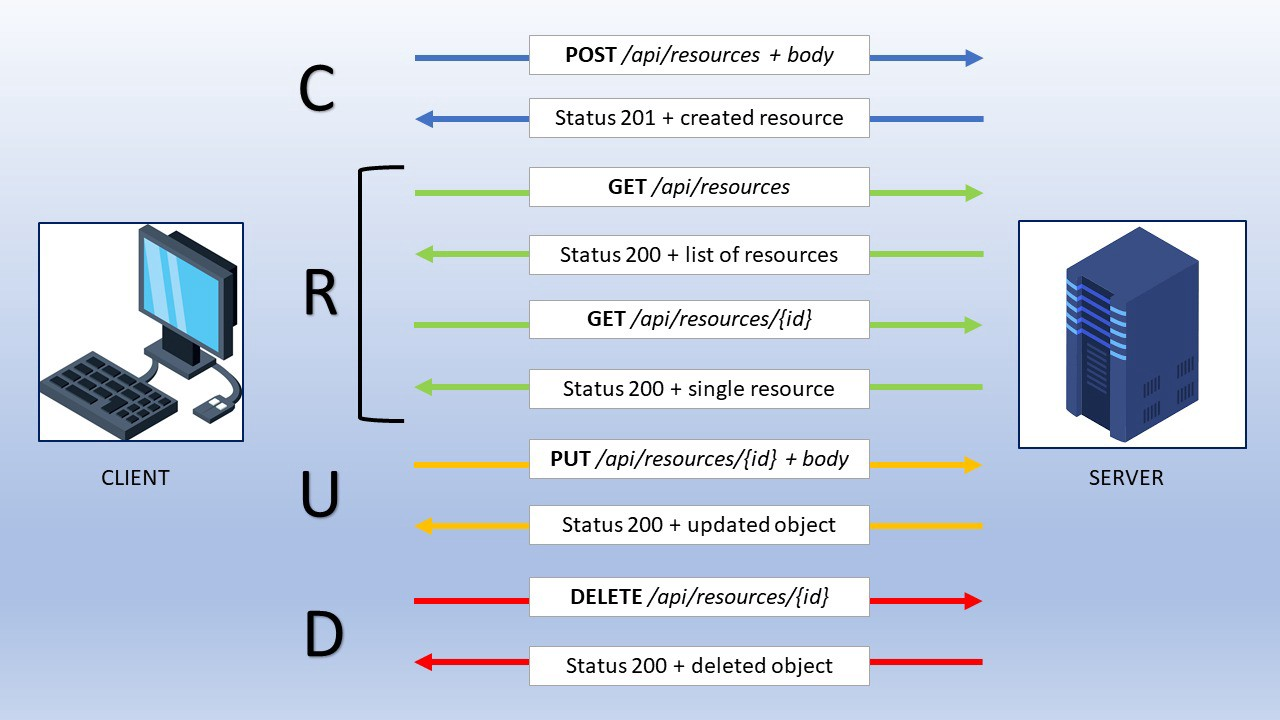
\includegraphics[width=\textwidth]{Figures/1. Tutorial/crud_guidelines.jpeg}
    \captionof{figure}{Princípios CRUD}
    \label{fig: crud guidelines}
\end{figure}

No diagrama acima é possível visualizar como as várias rotas devem ser estruturados para todas as operações (Criar, Ler, Atualizar, e Apagar) e o que cada um deles deverá retornar. De acordo com estes princípios, vamos separar as nossas rotas em dois ficheiros, um para especificar as rotas e o outro para definir o seu comportamento, isto é, as funções que irão fazer as operações reais e devolver a resposta certa a partir das rotas.

\subsubsection{Definindo as Rotas (Endpoints)}

Dentro da nossa pasta \texttt{src}, vamos agora criar uma nova pasta \texttt{routes}, com um ficheiro \texttt{products.routes.js} dentro. No terminal, vamos escrever o seguinte:

\lstinputlisting[language=SH, caption=Comandos para criar as rotas]{Listings/1. Tutorial/create_routes.sh}

Neste ficheiro iremos exportar uma função que leva três parâmetro: a aplicação Fastify, e devolve uma lista de rotas a serem adicionadas à aplicação. Especificamos o verbo HTTP a ser tratado, um URL, e, finalmente, uma função \textit{handler}, que iremos construir numa fase posterior, para cada rota.

\lstinputlisting[language=ES6, caption=Ficheiro models/products.routes.js]{Listings/1. Tutorial/routes_products_1.js}

Com estas rotas, somos agora capazes de realizar uma chamada HTTP do tipo:

\begin{itemize}
    \item \textbf{POST} à rota \texttt{api/products} para Criar um produto
    \item \textbf{GET} à rota \texttt{api/products} para obter uma Lista de todos os produtos
    \item \textbf{GET} à rota \texttt{api/products/:id} para Obter os detalhes de um dado produto
    \item \textbf{PATCH} à rota \texttt{api/products/:id} para Atualizar um dado produto
    \item \textbf{DELETE} à rota \texttt{api/products/:id} para Apagar um dado produto
\end{itemize}

O \texttt{:id} é um \textit{placeholder} para o identificador do nosso documento, permitindo-nos assim aceder ao mesmo através dos parâmetros de entrada do nosso pedido HTTP, na prática utilizando \texttt{request.params.id}.

Vale notar que por pré-definição o Fastify aceita apenas JSON (\texttt{application/json}) como tipo de entrada para o \texttt{body}. É possível adicionar suporte ao tipo de dados de um formulário HTML comum (\texttt{application/x-www-form-urlencoded}) bastando para isso adicionar o \textit{plugin} \textbf{@fastify/formbody} \cite{noauthor_fastifyformbody_nodate}, demonstrado na secção ???. à semelhança do \textbf{Express.js} também é possível suportar o carregamento de ficheiros através do \texttt{multipart/form-data} recorrendo ao \textit{plugin} \textbf{@fastify/multipart} \cite{noauthor_fastifymultipart_nodate}, não abordado neste tutorial.

Como visto acima, precisamos de acesso ao objeto da aplicação fastify para executar os manipuladores das rotas sobre ele, por isso devemos importar este ficheiro para o nosso \texttt{src/index.js} e chamá-lo com o app fastify como seu parâmetro. O Fastify permite-nos registar rotas através da função \texttt{app.register()} e definir prefixos para as mesmas, o que poderemos utilizar para simplificar a nomeação das nossas rotas e evitar erros. Deste modo, começamos por definir um roteador geral para a aplicação com o prefixo \texttt{"/api"} e dentro dele registamos um novo roteador para os nossos produtos que fará uso do nosso ficheiro de rotas e terá o prefixo \texttt{"/products"}. Resultado das alterações ao ficheiro \texttt{src/index.js} em seguida:

\lstinputlisting[language=ES6, caption=Ficheiro index.js atualizado com as rotas]{Listings/1. Tutorial/index_2.js}

\subsubsection{Definindo os Controladoras (Handlers)}

Depois de termos definido as nossas rotas, teremos de definir \textit{handlers} para cada uma delas. Por uma questão de simplicidade deslocaremos as nossas funções de manipulação para um ficheiro externo, onde criaremos a lógica necessária e a exportaremos e as designaremos para as suas respetivas rotas. Estes ficheiros são referidos como controladores. Como primeiro passo, estabelecer uma pasta de controladores no nosso diretório \texttt{src} e adicionar um novo ficheiro intitulado \texttt{products.controller.js}. Vamos abrir o nosso terminal dentro da pasta raiz do projeto e escrever:

\lstinputlisting[language=SH, caption=Comandos para criar os controladores]{Listings/1. Tutorial/create_controllers.sh}

Vamos agora trabalhar no novo controlador:

\lstinputlisting[language=ES6, caption=Ficheiro controllers/products.controller.js]{Listings/1. Tutorial/controller_products_1.js}

Antes de mais, temos de importar o nosso modelo de Produto, que será utilizado para realizar as transações na base de dados utilizando os métodos do Mongoose. Construímos então uma função para cada operação e marcámos-los como assíncronos, porque a nossa base de dados exigirá algum tempo para completar o seu processamento e não poderemos continuaras nossas operações enquanto tais pedidos não forem concluídos.

Vamos colocar a implementação dos \textit{handlers} em espera por agora e apenas conectar o nosso ficheiro de rotas a estas funções recentemente declaradas. Importamos o controlador e atribuímos as funções apropriadas dentro do ficheiro \texttt{products.routes.js}:

\lstinputlisting[language=ES6, caption=Ficheiro routes/products.routes.js atualizado com o controlador]{Listings/1. Tutorial/routes_products_2.js}

\subsection{Implementar os Controladores}

Vamos agora concentrar-nos em cada uma das nossas funções \textit{handler} dentro do \texttt{products.controller.js}.

\subsubsection{Criar um Produto}

Para criar um produto, devemos primeiro extrair informações do corpo (\texttt{request}) do pedido sobre o novo produto que vamos criar. Em seguida, utilizaremos o método \texttt{create} do Mongoose para criar um novo documento e devolvê-lo. Podemos agora definir o estado HTTP apropriado (201 Created) e devolver o nosso novo produto, de acordo com as convenções REST:

\lstinputlisting[language=ES6, caption=Função para criar um produto]{Listings/1. Tutorial/create_product.js}

\subsubsection{Obter a Lista de Proputos}

Esta é provavelmente a função mais simples. Receberemos o nosso pedido GET e executaremos a função de pesquisa no nosso modelo Product, passando um objeto vazio como parâmetro. O primeiro parâmetro é um objeto de consulta do MongoDB que especifica quais os produtos a obter com base em determinados critérios. Como resultado, o objeto vazio devolverá toda a coleção de produtos sem quaisquer restrições. Podemos então retornar os mesmos com o seguinte:

\lstinputlisting[language=ES6, caption=Função para listar os produtos]{Listings/1. Tutorial/list_products.js}

\subsubsection{Obter um Dado Produto}

O primeiro passo desta vez será obter o identificador único do produto que queremos do URL de pedido. Quando incluí-mos \texttt{placeholders} no URL da rota (como fizemos com o \texttt{:id} nas nossas rotas), eles aparecerão no objeto \texttt{request.params}. Após a obtenção do \texttt{id}, podemos utilizar o método \texttt{findById()} no modelo Product para recuperar o produto desejado, fornecendo o \texttt{id} como única parâmetro.

\lstinputlisting[language=ES6, caption=Função para obter um dado produto]{Listings/1. Tutorial/get_product.js}

\subsubsection{Atualizar um Produto}

A atualização implica que extraímos tanto o corpo do pedido como o identificador do produto do URL. As características do produto que necessitam de ser alteradas estarão no \texttt{body}, enquanto o \texttt{id} será utilizado para determinar qual o produto que precisa de ser atualizada. Podemos utilizar o método \texttt{findByIdAndUpdate()} com estas duas informações, fornecendo o \texttt{id} da nota como primeiro argumento e os dados do \texttt{body} como segundo argumento.

Ao contrário dos métodos \texttt{create}, \texttt{find} e \texttt{findById}, \texttt{findByIdAndUpdate} não devolve o objeto alterado por pré-definição, para alterar este comportamento é necessário fornecer um terceiro argumento à mesma, argumento este que deverá ser um objeto que defina a propriedade \texttt{"new"} como verdadeiro, de modo a que possamos responder com a nota recentemente alterada.

\lstinputlisting[language=ES6, caption=Função para atualizar um dado produto]{Listings/1. Tutorial/update_product.js}

\subsubsection{Apagar um Produto}

A eliminação de um produto será o último \texttt{handler} a ser feito. Neste caso não precisamos do \texttt{body}, tudo o que precisamos de fazer é obter o identificador do URL e fornecê-la ao método \texttt{findByIdAndDelete}. Esta função ao ser executada retorna o documento atual antes de eliminar o mesmo, pelo qual basta apenas devolve-lo na nossa resposta:

\lstinputlisting[language=ES6, caption=Função para apagar um dado produto]{Listings/1. Tutorial/delete_product.js}

\subsubsection{Controlador Final}

Pronto! Finaliza-mos o nosso ficheiro do controlador de produtos:

\lstinputlisting[language=ES6, caption=Ficheiro controller/products.controller.js atualizado com os handlers]{Listings/1. Tutorial/controller_products_2.js}

\subsection{Plugin @fastify/formbody}

O Fastify por pré-definição suporta apenas JSON no \texttt{body}. Este \textit{plugin} simples adiciona um \textit{parser} para o tipo de conteúdo \texttt{application/x-www-form-urlencoded}.

Primeiramente precisamos de instalar este plugin como uma dependência do nosso projeto:

\lstinputlisting[language=SH, caption=Comandos para a instalar o plugin @fastify/formbody]{Listings/1. Tutorial/install_formbody.sh}

Em Fastify podemos considerar que um \textit{Middleware} é um \textit{Plugin}, na realidade, à semelhança do JavaScript em que tudo é um objeto, em Fastify tudo é um \textit{plugin}. Para utilizar este \textit{plugin} na aplicação basta registar o mesmo na aplicação fastify:

\lstinputlisting[language=ES6, caption=Ficheiro index.js com @fastify/formbody]{Listings/1. Tutorial/index_3.js}
